\documentclass{article}
\usepackage[T1,T2A]{fontenc}
\usepackage[utf8]{inputenc}
\usepackage[english,russian]{babel}

\usepackage[left=3cm,right=3cm,
    top=3cm,bottom=3cm,bindingoffset=0cm]{geometry}

\usepackage{graphicx}
\usepackage{color}
\usepackage{hyperref}

\usepackage{setspace}
\usepackage{indentfirst}
\usepackage{textcomp}
\usepackage{ifthen}
\usepackage{calc}

\title{Теор. Вер.}
\author{Лекция 1}

\begin{document}
\maketitle

\section{Вступление}

Почта преподавателя: oaw804mai@yandex.ru

Будут три контрольных:

\begin{enumerate}
\item ... (где-то после 8 марта)
\item Cлучайные величины
\item Случайные векторы
\end{enumerate}

Вопросы, которые даются после лекции, требуется прорабатывать (письменно, с подписью листов), не оставляя до конца семестра.

\section{Классическая схема теории вероятностей (КСТВ)}

Мы будем иметь дело с \textbf{опытом}.

\textbf{Опыт} -- комплекс условий, который в неизменном виде может быть воспроизведен многократно.

То есть теория вероятностей изучает явления, которые носят массовый характер. К явлениям, которые производятся, 4-5 раз, в принципе нельзя применить теорию вероятностей.

Примером многократного опыта можно назвать классическое подбрасывание монетки (орел, решка). 

Результат многократного воспроизведения опыта -- это \textbf{исход}

\subsection{Элементарный исход}
\textbf{Определение.} Элементарный исход -- это элемент множества элементарных исходов опыта.

Само множество обозначаем "омега большое": $\Omega$.

Элементарные исходы удовлетворяют следующим условиям:

\begin{enumerate}
\item Количесво элементарных исходов опыта конечно;
\item Элементарные исходы попарно несовместны (при однократном воспроизведении опыта никакие два элементарных исхода одновременно не реализуются!);
\item Элементарные исходы образуют полную группу (при воспроизведении опыта реализуется один и только один из множества элементарных исходов -- никакие другие исходы невозможны);
\item Элементарные исходы равновозможны, никакому из них не отдается приоритет (кстати, четкой математической формулировки для равной возможности не существует).
\end{enumerate}

$\Omega = \{\omega_1, \omega_2, ..., \omega_N\}$

Где $N$ -- кол-во элементарных исходов опыта.

\subsubsection{Пример}

Бросают три монеты.
Мы хотим построить множество элементарных исходов опыта с бросанием трех монет.
Сами мы не будем воспроизводить опыт, но опишем то, что мы наблюдали бы при исполнении опыта.

Варианты с выпадением "орла" (шт): $0 , 1 , 2 , 3$. Эти варианты несовместны (не может быть два сразу), так что они образуют полную группу. Однако, наш опыт говорит о том, что данные варианты будут неравновероятны (чаще мы будем видеть результаты с 1-2 орлами). Тогда, попытаемся это исправить.

Пронумеруем монеты номерами, и укажем все дополнительные сведения для каждой монетки (номер-результат).

Примем $0$ -- за решку, а $1$ за орла. Имеем следующие монеты и элементарные исходы:

\begin{center}
1 2 3\\
-----\\
0 0 0\\
0 0 1\\
0 1 0\\
0 1 1\\
1 0 0\\
1 0 1\\
1 1 0\\
1 1 1\\
\end{center}

И заметим, следующее:

\begin{center}
0 орлов -- 1 исход\\
1 орел -- 3 исхода\\
2 орла -- 3 исхода\\
3 орла -- 1 исход\\
\end{center}

У нас получаются разные результаты, которым соответствуют различное количество элементарных исходов. Эти результаты получаются, очевидно, неравновероятными (но не стоит забывать, что все исходы равновозможны! Важно их количество.).

\subsection{Случайное событие}

\textbf{Определение.} Случайным событием в опыте с множеством элементарных исходов $\Omega$ является любое подмножество множества $\Omega$.

Сами события мы будем обозначать большими латинскими буквами: $A, B, ..., Z$, при этом $A \subseteq \Omega$.

$A$ \textbf{реализуется} в опыте, если реализуется хотя бы один элементарный исход, входящий в это событие.

Само событие обычно записывают в виде текста, заключенного в фигурные скобки:

$A = \{$ выпал один орел $\} = \{\omega_2, \omega_3, \omega_5\}$ (см элементарные исходы выше)

Все возможные события в опыте образуют \textbf{алгеброй событий} $\mathcal{A}$ -- множество всех подмножеств в множестве элементарных исходов $\Omega$:

$$ \mathcal{A} = 2^{\Omega} $$

\textbf{замечание}: иногда случайным событием называт что-то, что происходит или не происходит. Это утверждение неверное. Случайным событием в опыте является только элемент в алгебре событий.
В опыте может рассматриваться ситуация, когда в опыте что-то просиходит или не происходит, но эта ситуация в алгебру событий не входит. Такое явление не является частью теории вероятностей, поскольку с ним нельзя связать никакой числовой величины.

\subsection{Вероятности}

\textbf{Определение.} Вероятностью случайного события $A$ в опыте называется отношение:
$$ P(A) = \frac{N_A}{N},$$
где $N_A$ -- колво элементарных исходов в событии А (количество элементарных исходов, благоприятствующих событию А),
$N$ -- колво элементарных исходов в опыте (всего).

То есть каждому событию мы сопостовляем число и называем это число \textbf{вероятностью} события.

\textbf{Следствие}: вероятность величина \textbf{ограниченная}:

$$ 0 \leq P(A) \leq 1 $$

\quad

Событие, не реализующее ни один элементарный исход: $\emptyset \in \mathcal{A} $ -- называется невозможном событим $\Rightarrow P(\emptyset) = 0$.

Событие, реализующее все множество элементарных исходов: $\Omega \in \mathcal{A}  $ -- называется достоверным $\Rightarrow P(\Omega) = 1$

\subsection{Комбинации событий}
\subsubsection{Сумма событий}

\textbf{Определение.} Сумма событий $ A + B $ -- это событие, состоящее в том,что происходит одно из событий A или B $\rightarrow (A\cup B) $.
\subsubsection{Произведение событий}

\textbf{Определение.} Произведение событий $AB$ -- это событие, состоящее в том, что происходит каждое из событий A и B $\rightarrow(A\cap B)$.

\subsubsection{Потивополоэное событие}

\textbf{Определение.} Противоположное событие $\overline A$ -- событие, состоящее в том, что событие $A$ не происходит.

\subsection{Несовместные и несовместные события}

Случайные события называются несовместными, если они не происходят одновременно. То есть $AB = \emptyset$.

В остальных случаях события называются совместными.

\quad

Для несовместных событий $A$ и $B$: $P(A + B) = P(A) + P(B)$

В общем случае: $P(A + B) = P(A) + P(B) - P(AB) $

Для событий $\overline A$: $P(\overline A) = 1 - P(A)$

\subsection{Геометрические вероятности}

Цель: понять, от каких условий КСТВ можно отказаться.

Можно попробовать отказаться от конечности элементарных исходов опыта (условие №1). Например, можем связать исход в измеримой величиной объекта (площадь, объем), но от остальных условий в этом случае отказаться мы не получится.

Тогда мы моэжем определить вероятность события как отношение некоторых характеристик:

$$ P(A) = \frac{m(A)}{m(\Omega)};$$

где $m(\cdot)$ -- длина (площадь, объем, вес...).

\subsection{Примеры}
\subsubsection{Пример 1}

Два студента договорились встретиться от 12 часов до 13. Любой из них, придя на эту встречу, ждет товарища 20 минут и после этого уходит. Какова вероятность встречи студентов в этих условиях?

Проблема: у каждого студента есть свое время прихода $t_1$ И $t_2$. По КСТВ мы не можем это сделать, так как количество элементарных исходов не конечно (оно, в общем-то, даже не счетно).

Сделаем следующее: введем систему координат. По одной, отложим момент прихода одного студента, по другой -- момент прихода второго студента.

\begin{center}
    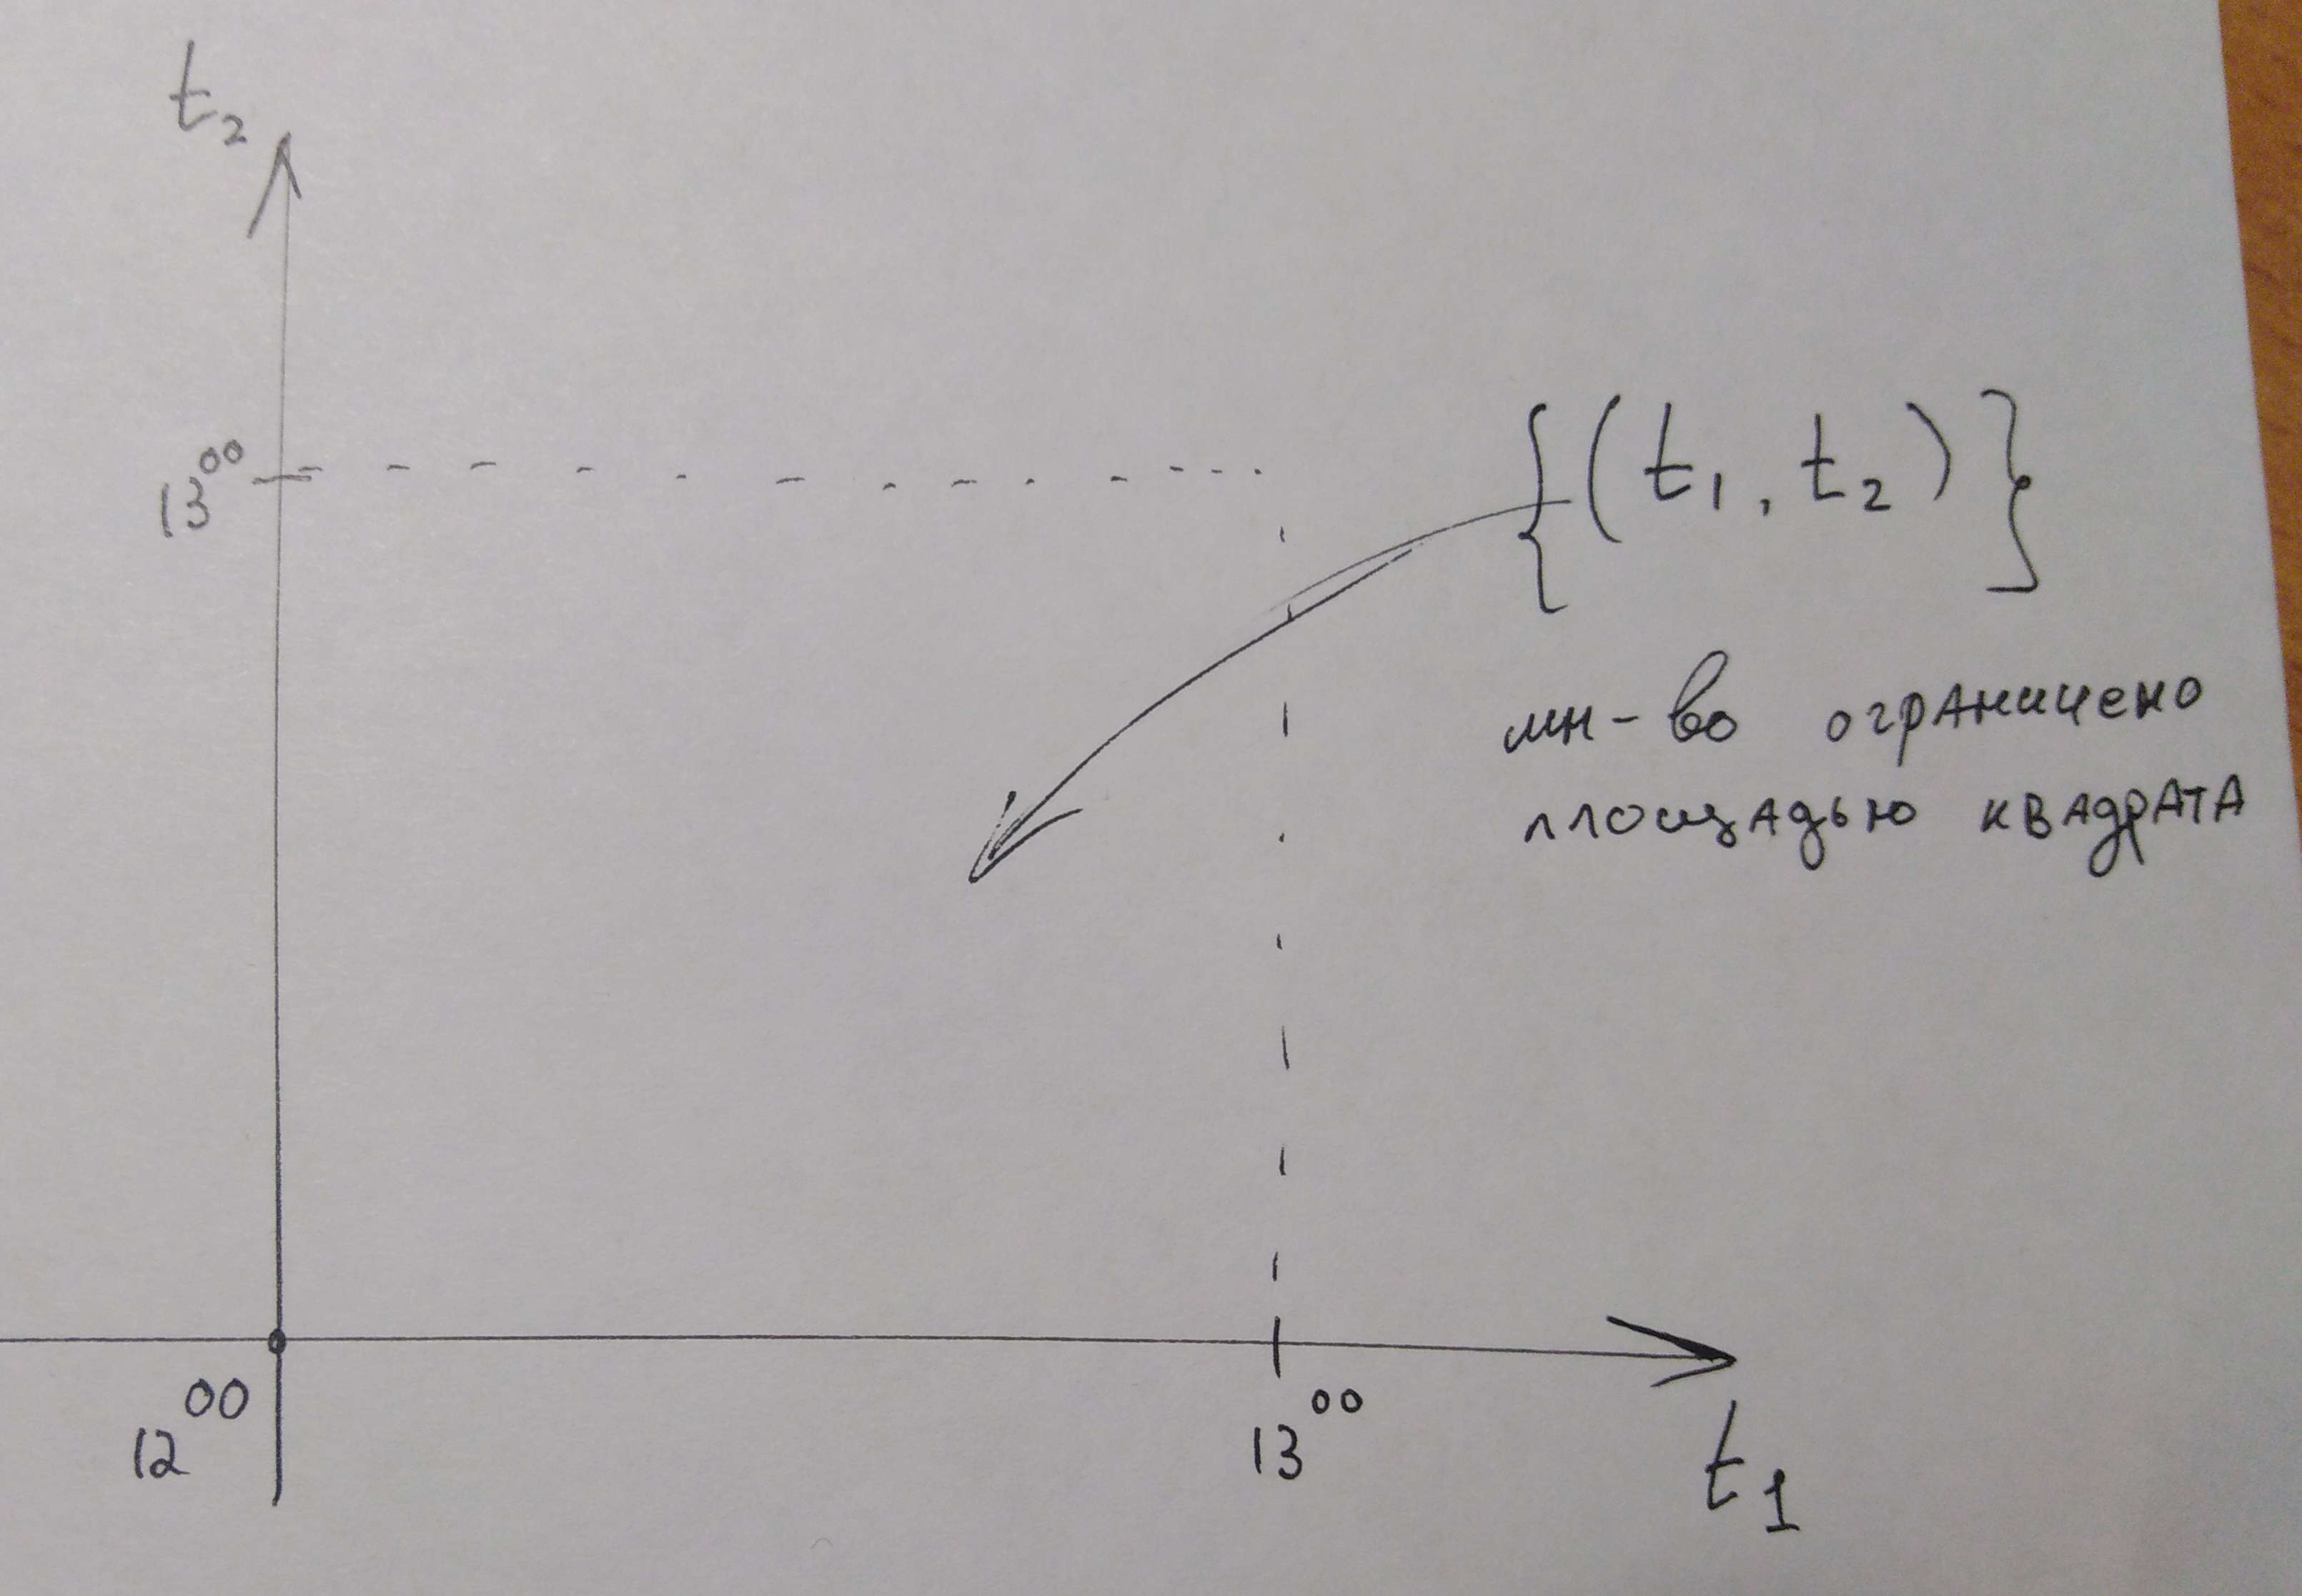
\includegraphics[scale=0.16]{1_1.jpg}
\end{center}

При этом множество всевозможных точек $(t_1, t_2)$ ограничено площадью квадрата времени от 12 до 13.

Обозначим событие $B = \{$ встреча состоялась $\} = \{(t_1, t_2) : |t_1 - t_2| \leq \frac{1}{3}\}$ ($\frac{1}{3}$ так как доступное время встречи -- 20 минут, треть от часа).

\begin{center}
    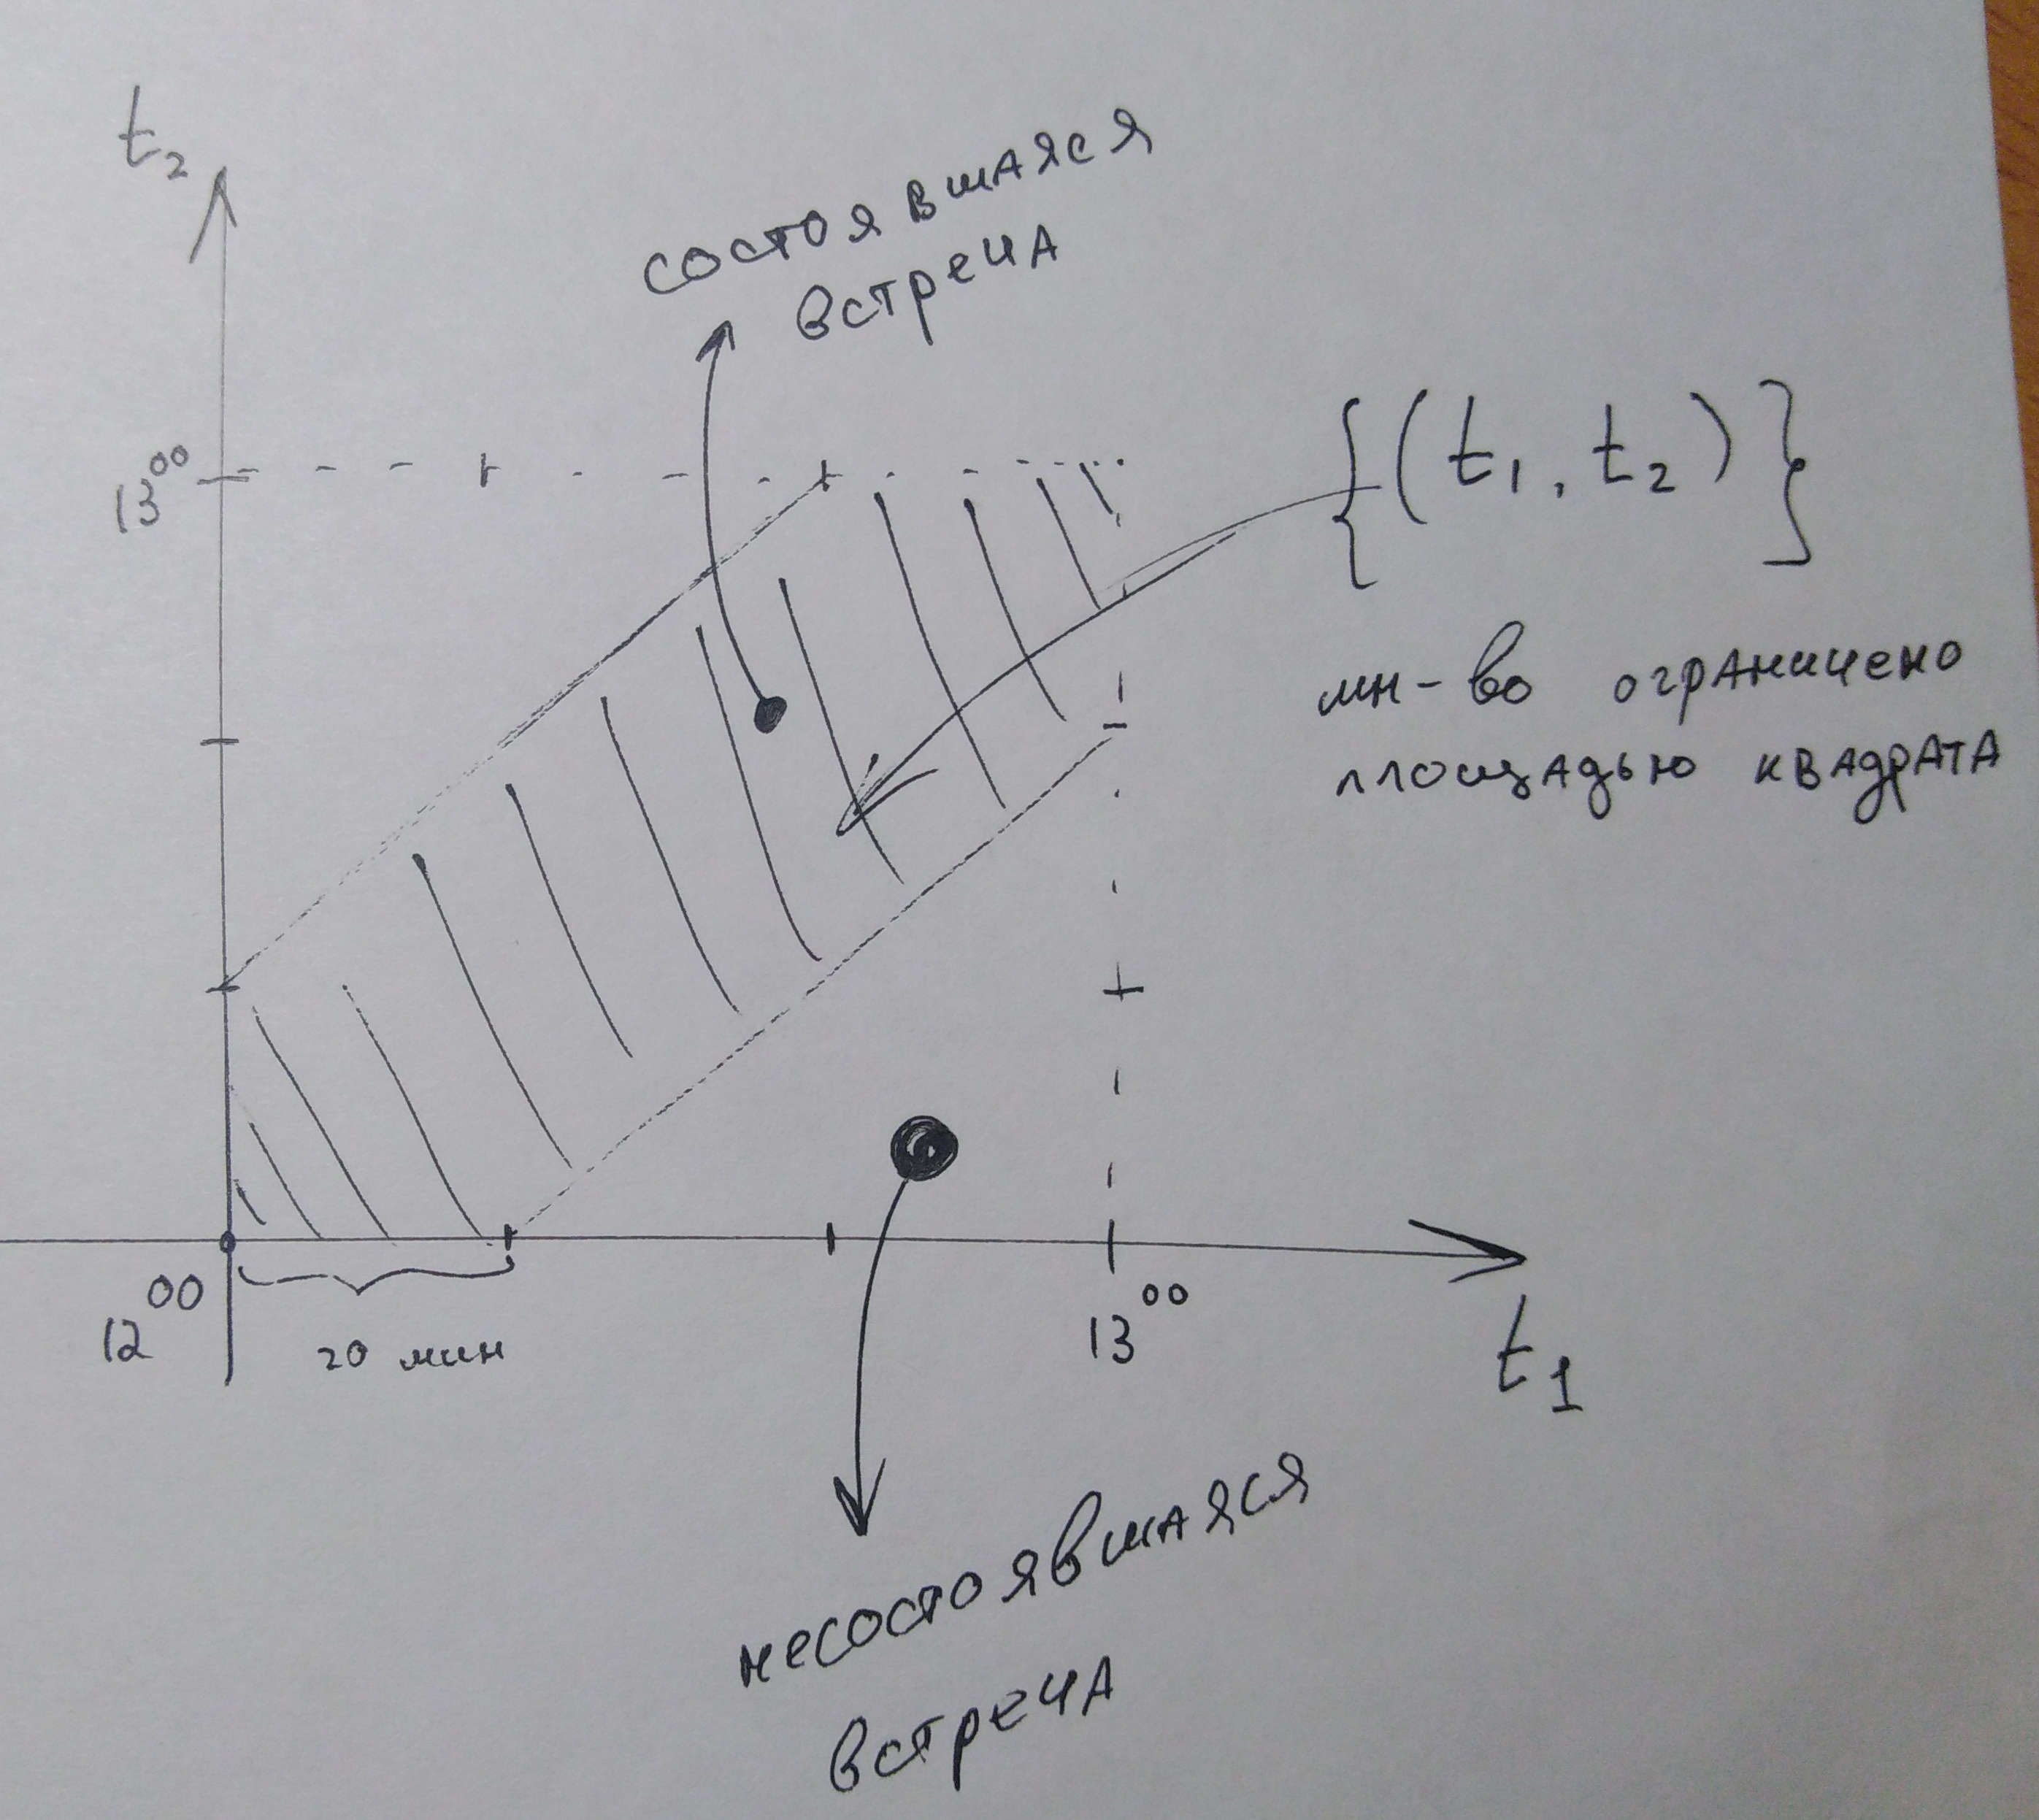
\includegraphics[scale=0.2]{1_2.jpg}
\end{center}

В итоге, мы получаем закрашенную область, в котором встреча состоится. Таким образом, вероятность выполнения события $B$ является отношением площадей:

$$P(B) = \frac{S_B}{S_{\Omega}} = \frac{1 - 2 * \frac{1}{2} * \frac{2}{3} * \frac{2}{3}}{1} = \frac{5}{9} $$

Можно заметить, что несмотря на странность условий, вероятность состоявшейся встречи больше половины!

\subsubsection{Пример 2}

Имеем: $m$ белых шаров и $n$ черных ($m \neq n$). Шары в урне.
Наугад берут один шар. Какова вероятность того, что шар -- белый?

Пронумеруем шар. Тогда общее число элементарных исходов $N = m + n$.

Событие $A = \{$ шар белый $\} \rightarrow N_A = m$

Соответственно, $P(A) = \frac{m}{m + n}$.

\subsubsection{Пример 3}

Те же белые и черные шары, но их наугад раскладывают в ряд. С какой вероятностью на $k$-ом месте ($1 \leq k \leq m + n$) в этом ряду будет белый шар?

Ответ, на самом-то деле, такой же: $\frac{m}{m + n}$. Но как мы его получили?

Шары пронумерованы. Значит, общее количество всех возможных исходов $N = (m + n)!$ (колво перестановок).

Колво благоприятных вариантов $N_A = m * (m + n - 1)!$.

$P(A) = \frac{N_A}{N} = \frac{m}{m + n}$.

\textbf{Замечание.} Можно не только было пронумеровать шары, можно было опыт построить по другому. Расстановка шаров в ярду -- наугад. Берем шар, ставим на первое, берем шар, ставим на второе... Шары стоят наугад. Но шары можно заполнять и в произвольном порядке по свободным местам (в начало, конец, середину). Но это означает, что мы можем начинать произвольное место, в том числе с $k$-ого, то есть остальные шары нам не нужны для ответа. И по сути получается предыдущая задача.

Но самое главное, что на самом-то деле от номера места ничего не зависит. Независимо от номера места, вероятность останется той же.

\subsubsection{Пример 4}

Та же ситуация, но поменяем состав шаров: $m$ белых, $n$ черных, $k$ желтых. Шары разложены в ряд наугад. С какой вероятностью белый шар в этом ряду встретится раньше черного?

Не очень-то смешно, но ответ тот же: $\frac{m}{m + n}$.

Шары нумеровать \textbf{не} будем. Сколько будет способов расставить шары в ряд, если номеров нет?

Всего в ряду $m + n + k$ мест. Так как желтые особо никак не мешают нам, расставим сначала их:

$N = C_{m + n + k}^k * C_{m + n}^m$

Наконец подсчитаем количество благоприятных исходов:

$N_A = C_{m + n + k}^k * 1 * C_{m + n - 1}^{m - 1}$ (черные шары нет необходимости расставлять, они просто займут оставшиеся места)

В итоге при делении получится требуемый ответ.

\subsubsection{Итог}

Несмотря на одинаковость ответов, самое важное -- решение. Именно оно важно, в том числе при выполнении дз.

\end{document}
